\documentclass[pdftex,aspectratio=169]{beamer}

% Setup UTF-8 encoding
\usepackage[utf8]{inputenc}
\usepackage[T1]{fontenc}

%\usepackage{flashmovie}

% Setup beamer look theme
\mode<presentation>
{
	\useinnertheme{rectangles}
	\useoutertheme{infolines}
%	\usecolortheme{crane}
%	\usecolortheme{dove}
	\usecolortheme{seagull}
	\setbeamertemplate{navigation symbols}{}
}

% Use nicer font
\usepackage{palatino}
\usepackage{palatino,graphics,array}


% Setup czech language
\usepackage[czech]{babel}

% Include usefull packages
\usepackage{graphics}

% Include hyperlinks support
\usepackage{hyperref}
\hypersetup{colorlinks=true,linkcolor=black,urlcolor=black,unicode=true}

% Add support for simple URLs
\usepackage{url}

\usepackage{tikz}

\usepackage{verbatim}
\usetikzlibrary{arrows,shapes}
\usetikzlibrary{mindmap,trees}


% Commands for CC license
\newcommand{\CcLongnameByNcSa}{\href{http://creativecommons.org/licenses/by-nc-sa/3.0/cz/}{Attribution-Noncommercial-ShareAlike}}
\newcommand{\CcImageBy}[1]{
\includegraphics[scale=#1]{graphics/cc-by-white.pdf}}
\newcommand{\CcImageNc}[1]{
\includegraphics[scale=#1]{graphics/cc-nc-white.pdf}}
\newcommand{\CcImageSa}[1]{
\includegraphics[scale=#1]{graphics/cc-sa-white.pdf}}
\newcommand{\CcGroupByNcSa}[2]{\CcImageBy{#1}\hspace*{#2}\CcImageNc{#1}\hspace*{#2}\CcImageSa{#1}}




\title{Scheduling the GRID(s)}
\subtitle{an introduction}
\author[]{Mgr.~Šimon~Tóth}
\institute[FI@MU]{Fakulta informatiky @ Masarykova Univerzita}
\date{\today}

\newcommand{\CcNote}[1]{% longname
        Licencováno pod: \textit{Creative Commons #1 3.0 License}.%
}

\begin{document}

\pgfdeclarelayer{background}
\pgfsetlayers{background,main}

\begin{frame}
\titlepage
	\vfill
	\begin{center}
		\CcGroupByNcSa{0.33}{0.95ex}\\ {\tiny\CcNote{\CcLongnameByNcSa}}
		\vspace*{2ex}
	\end{center}
\end{frame}

% Thank you all for comming here. My name is Simon Toth and I would like to
% introduce you today into the area of grid scheduling, with particular
% emphasis on distributed scheduling.

% Because this is my first year of PhD studies, I will be mostly trying to
% introduce you into the area of grid scheduling and the challenges we are
% facing.

{
\usebackgroundtemplate{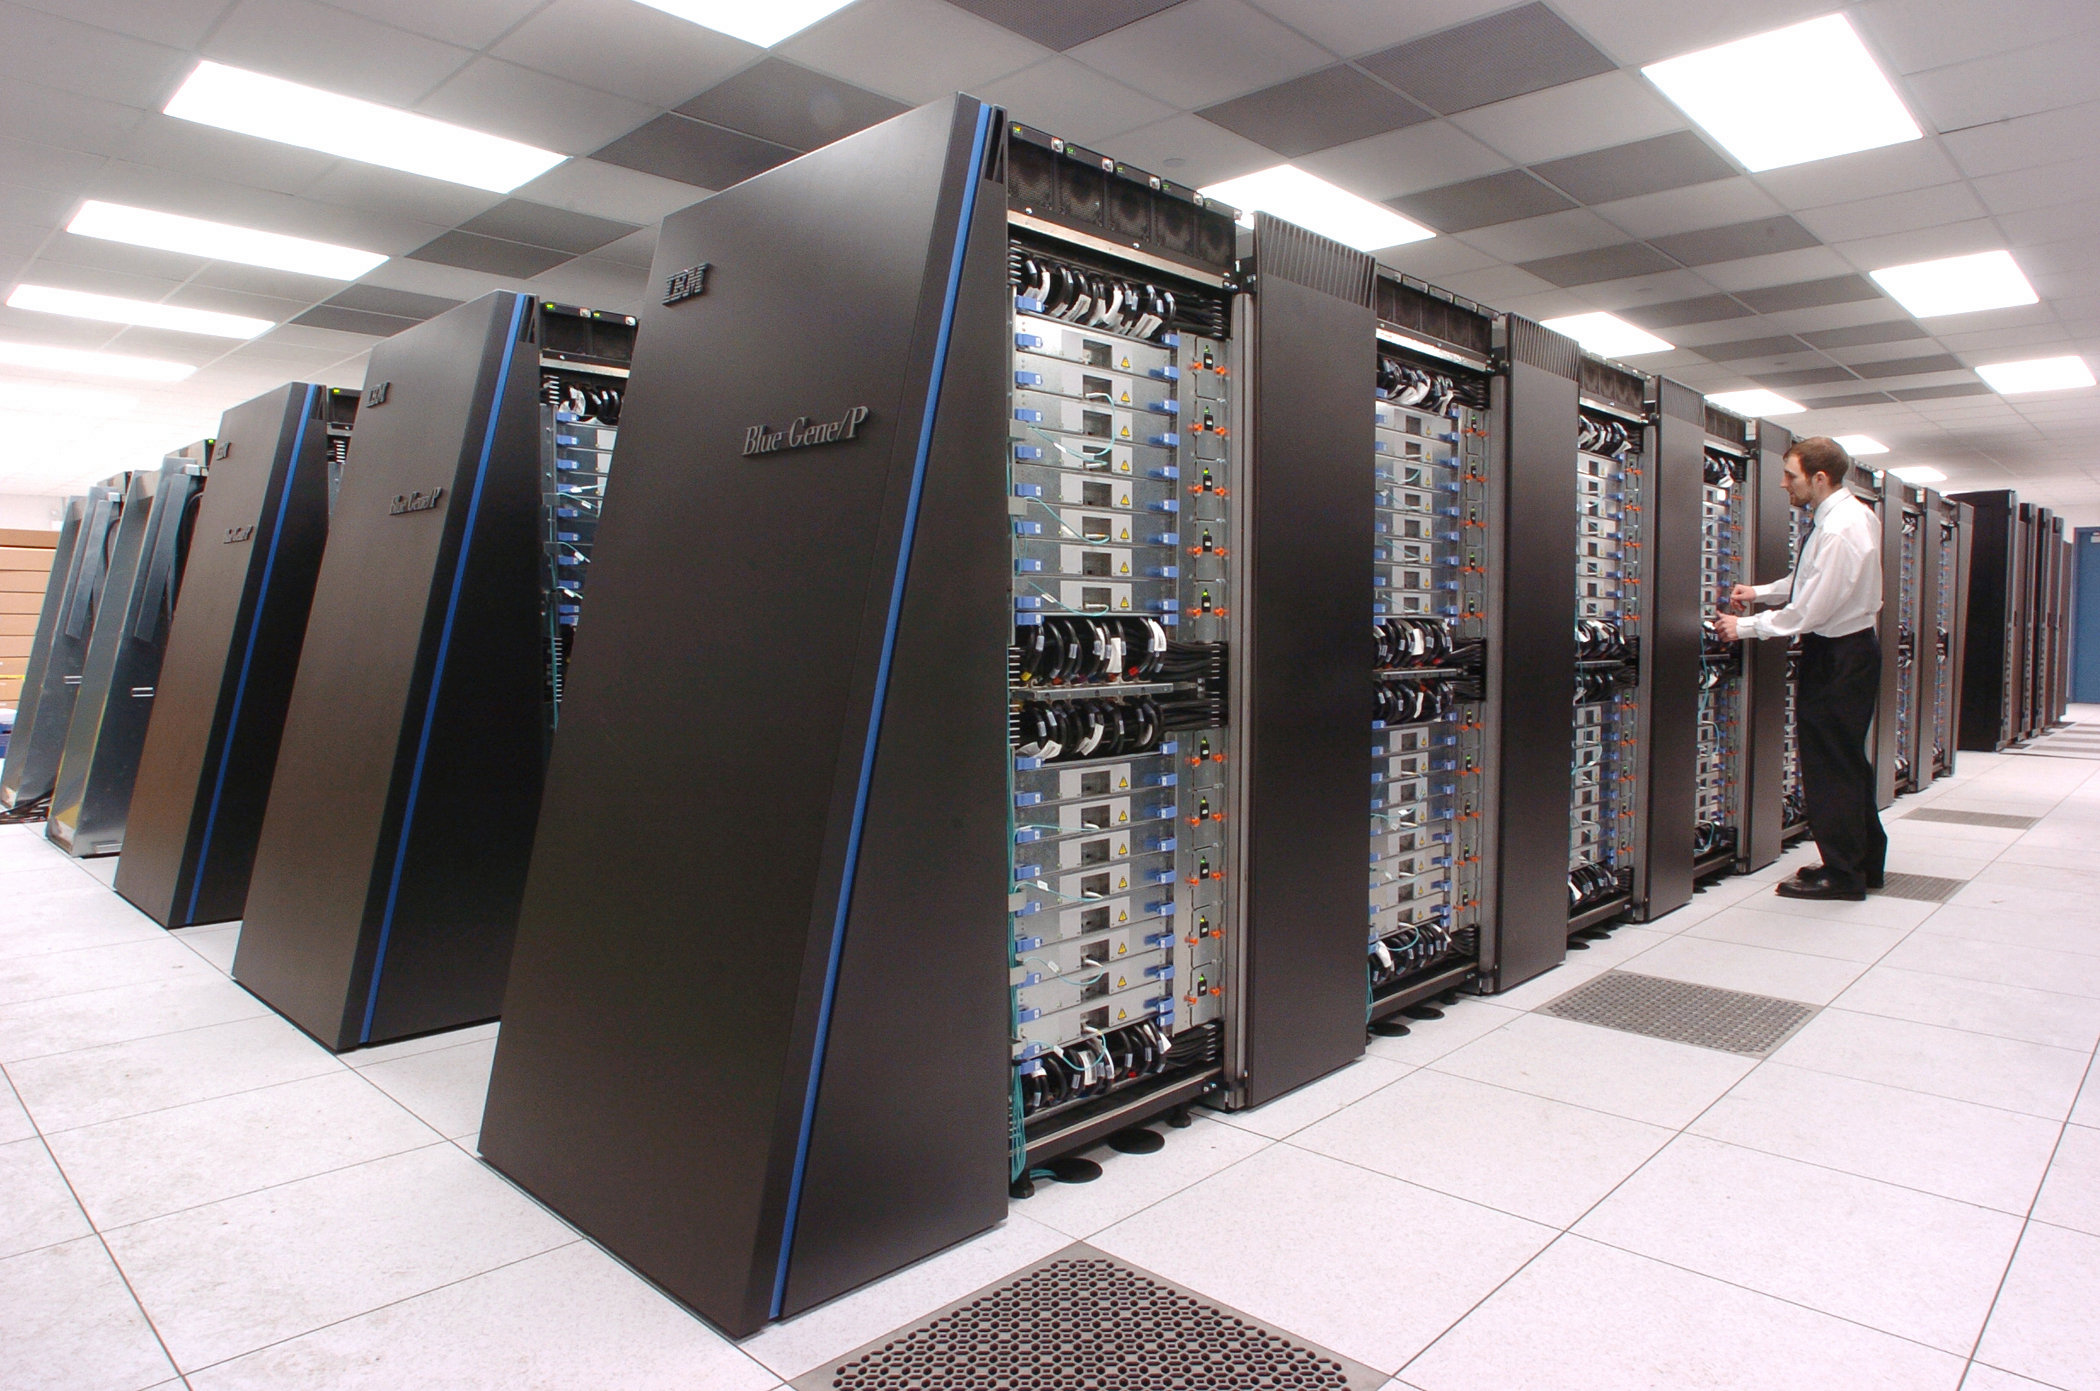
\includegraphics[width=\paperwidth]{imgs/ibm-blue-gene.jpg}}
\frame{}
}

{
\usebackgroundtemplate{
\includegraphics[width=\paperwidth]{imgs/ibm-blue-gene-back.jpg}}
\begin{frame}

% Now please allow me a short quiz before we really start
% Who of you knows what is a grid?
% Who of you heard either about MetaCentrum or Cerit?
% Who of you actually used a grid?

	\begin{columns}
	\column{0.45\textwidth}
	\begin{block}{Hardware models}
	\begin{overlayarea}{\textwidth}{4cm}
		\begin{itemize}
			\item<1->{super-computer}
			\item<2->{computer cluster}
			\item<3->{computational grid}
			\item<4->{scientific cloud}
		\end{itemize}
		\vspace{5cm}
	\end{overlayarea}
	\end{block}

	\column{0.45\textwidth}
	\begin{block}{Features}
	\begin{overlayarea}{\textwidth}{4cm}
	% when you are buing a supercomputer, you are either shooting for maximum possible performance, or you have a specific use case and some rough estimate of required computing power
	% supercomputers, aren't usually suitable for generic computing, usually, they are optimized for a spefic use case scenario
	% they also tend to be expensive
	% and they usually run specialized software, upto the point of providing special implementations of language (and other) libraries
	\only<1>{
	\small
	\begin{itemize}
		\item maximum/specific performance
		\item not suitable for generic computing
		\item expensive
	\end{itemize}
	}
	% the basic idea of a cluster is that instead of buing an expensive supercomputer you buy a "cluster" of homogenous machines and
	% interconnect them into a computer network
	% when buying a cluster you are usually targeting the sweetspot of maximum performance to price ratio
	\only<2>{
	\small
	\begin{itemize}
		\item maximum performance to price ratio
		\item homogenous environemnt
	\end{itemize}
	}
	% now with clusters, you can get nice performance for reasonable price
	% but still, specifically when your requirements are specific, you usually can't satisfy all users
	% when you for example buy a cluster with GPU cards, you can't really expect this cluster to have great raw CPU performance
	% this is where grids come into play
	% in grids we are starting to distinguish multiple parties
	% first there are the resource providers, these provide computing and storage facilities for the users
	% then there are virtual organizations, these are mostly groups of users, but with their own "organizational structure"
	% virtual organizations then negotiate access to resources for their users
	\only<3>{
	\small
	\begin{itemize}
		\item maximum utility
		\item heterogenous environment
	\end{itemize}
	}
	% the latest member to the family of computing architectures is cloud computing
	% now this is a strage member, since cloud isn't really an architecture, it's a sales model
	% right now, the majority of the computing cost is in the hardware and in electricity
	% therefore it makes sense to sell access per CPU hour
	\only<4>{
	\small
	\begin{itemize}
		\item maximum financial gain
		\item dynamic environment
	\end{itemize}
	}
	\vspace{5cm}
	\end{overlayarea}
	\end{block}
	\end{columns}

\end{frame}

\begin{frame}

\end{frame}
}

% To explain to you what we are doing, please allow me to introduce a marketplace metaphor.
% Let's imagine a marketplace. And not just any marketplace, a marketplace with very demanding clientele.
% First of all, customers don't want to waste their time and only want to enter the marketplace when their requirements can be fulfilled.
% Secondly, some of the customers don't want to even waste time shoping, and just want to hand-in a list of requirements with an address to ship them to.

% Now for such system to work you need one entry point to the marketplace with some entity maintaining information about the current state of the marketplace.
{
\usebackgroundtemplate{
\includegraphics[width=\paperwidth]{imgs/marketplace.jpg}}
\frame{}
}



\begin{frame}
	\frametitle{Cloud}

	cloud computing
	CPU time billing model
	high flexibility, dynamic infrastructure
	immediate scalability
\end{frame}


\section{Scheduling on grids}

\begin{frame}
	\frametitle{Scheduling on Grids}
	ukazka planovani jobu pro minimalizaci slowdown - dynamicke programovani
	vysvetleni problemu non-clairvoirance
	planovani bez zname delky jobu
	vysvetleni problemu on-line scheduling
\end{frame}

% lack of criteria
%	non-comparability of solutions

\section{Current approaches}
\subsection{FIFO based solutions}
\subsection{Schedule based solutions}

% FIFO based solutions
%	jobs are processed on a first-come first-serve basis
%	mutliple extensions using priorities, jobs starvations, etc...
%	easy to grasp, hard to manage (each configuration option affects all other configuration options)
%	can be very britle

% Schedule based solutions
%	the scheduler creates a real job schedule
%	scalability and performance issues
%	problems with very dynamic configurations

% Scalability and stability
% 

% Approaching the distributed environment
%	bin packing

% Deadline scheduling

% One of the possible approaches that could allow us to escape the current rigid model is deadline scheduling.
% In deadline scheduling, the scheduler is trying to create a schedule that will violate the least amount of deadlines.
% We are depending largely on the information provided by the oracle, since we don't have any other source of precise job runtime.

















\end{document}
